\section{Variationen / Erweiterungen zu PID-Reglern}

\subsection{Modifizierter PID-Regler in Parallelform}{171}

\begin{minipage}[t]{0.4\columnwidth}
    \begin{center}
        \textbf{\myul{Parallelform (normal)}}
    \end{center}
    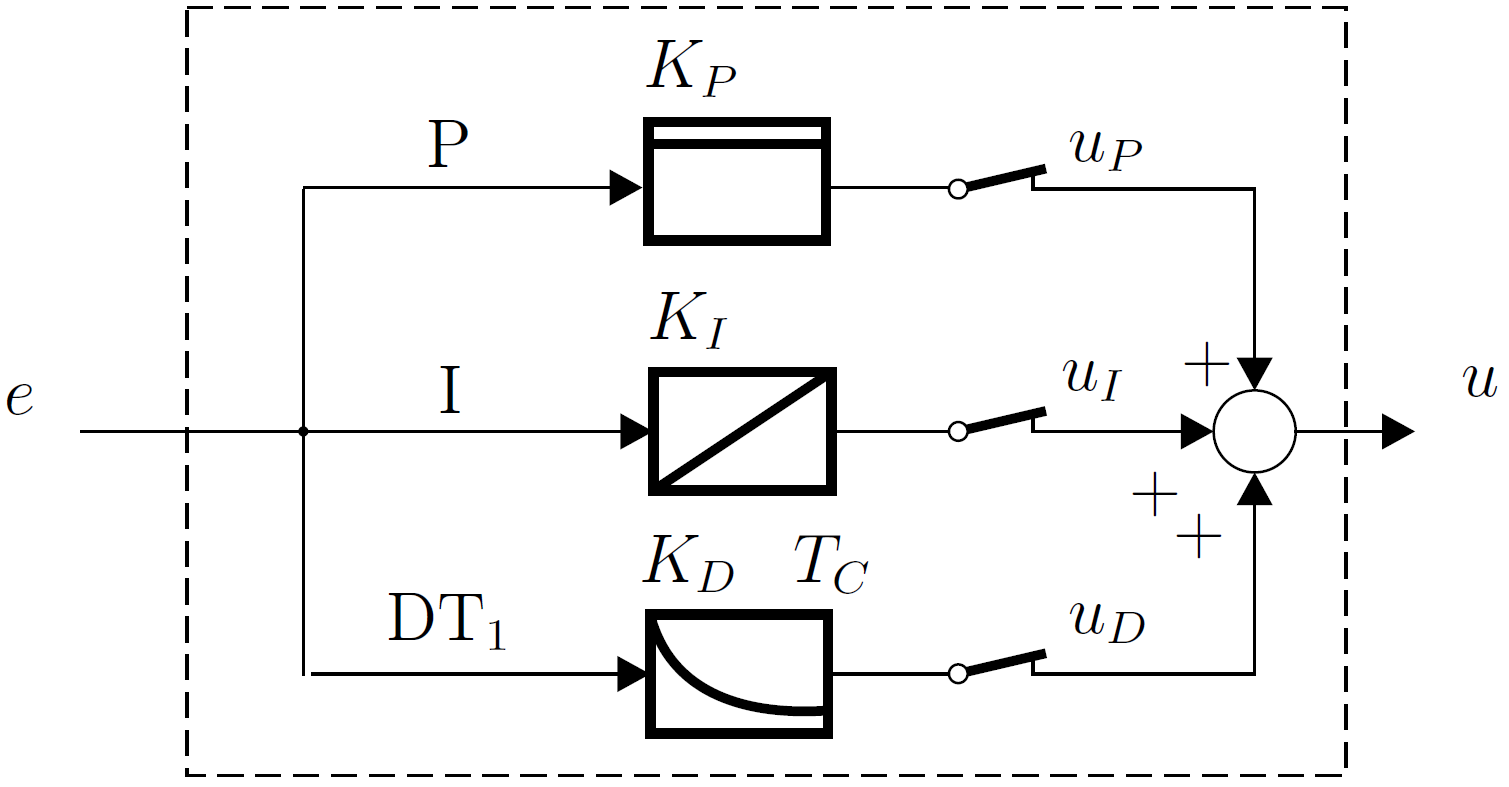
\includegraphics[width=\columnwidth]{images/pid_regler_aufbau.png}

    \textbf{Hinweis:} $P$-Anteil darf auch nach vorne gezogen werden (wie links) 
    \textrightarrow\ ändert Parameter von $I$- und $\text{DT}_1$-Gliedern
\end{minipage}
\hfill
\begin{minipage}[t]{0.55\columnwidth}
    \begin{center}
        \textbf{\myul{Modifizierte Form}}
    \end{center}
    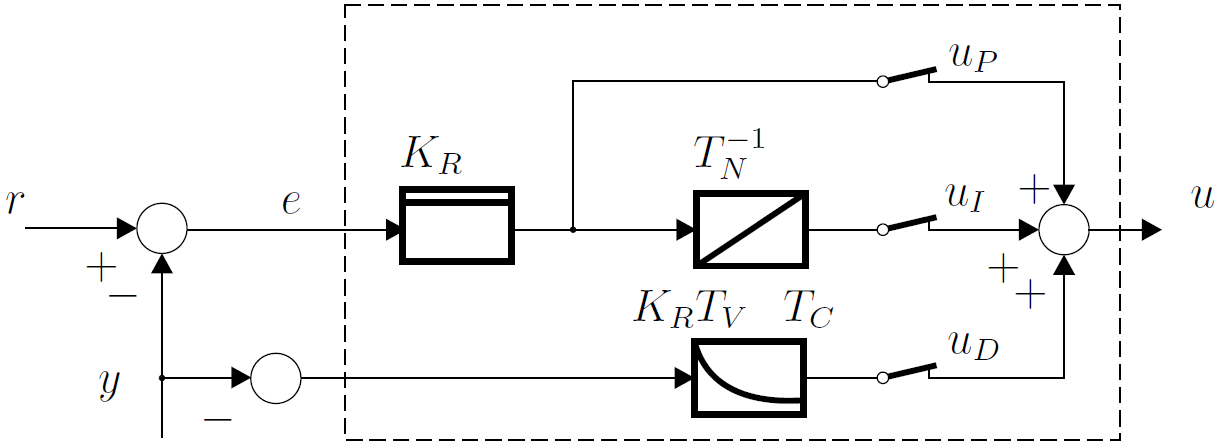
\includegraphics[width=\columnwidth]{images/modifizierter_pid_regler.png}

    Statt Fehler $e$ wird Ausgang $y$ auf $\text{DT}_1$-Glied geführt! \\
    \textrightarrow\ Ableitung des Ausgangs $y$ statt Ableitung des Fehlers $e$
\end{minipage}


\subsubsection{Eigenschaften / Auswirkungen der Modifikation}

\begin{minipage}[t]{0.48\columnwidth}
    \raggedright
    \begin{center}
        \textbf{\myul{Parallelform (normal)}}
    \end{center}

    \begin{outline}
        \1 Ändernde Referenz $r(t)$ (z.B. Sprung)
            \2 $\text{DT}_1$-Glied reagiert sehr aggressiv, da $e(t)$ gross \\
                \textrightarrow\ 'Überforderung' des Stellglieds
    \end{outline}

\end{minipage}
\hfill
\begin{minipage}[t]{0.48\columnwidth}
    \raggedright
    \begin{center}
        \textbf{\myul{Modifizierte Form}}
    \end{center}

    \begin{outline}
        \1 Ändernde Referenz $r(t)$ (z.B. Sprung)
            \2 $\text{DT}_1$-Glied reagiert nicht so aggressiv, da $y(t)$ 'träger' als $e(t)$ \\
                \textrightarrow\  Stellglied 'geschont'
        \1 'two degrees of freedom'
            \2 Reaktion auf Störung bzw. auf Änderung der Referenz separat einstellbar
    \end{outline}
\end{minipage}

\textbf{Achtung:} Der $\text{DT}_1$-Anteil kann nicht einfach weggelassen werden! 


\subsection{Glättung der Referenz}{171}

\begin{minipage}[c]{0.3\columnwidth}
    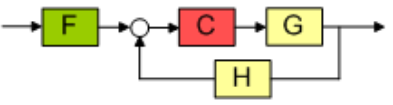
\includegraphics[width=\columnwidth]{images/filterung_stellgroesse.png}
    % \begin{center}
    \scalebox{0.4}{
    \begin{tikzpicture}
        [
            scale = 1,
            >=latex,
            orangebox/.style={rectangle, draw=black, fill=orange, thick, minimum width=1cm, minimum height=0.5cm},
            greenbox/.style={rectangle, draw=black, fill=green, thick, minimum width=1cm, minimum height=0.5cm},
            yellowbox/.style={rectangle, draw=black, fill=yellow, thick, minimum width=1cm, minimum height=0.5cm},
            whitecircle/.style={circle, draw=black, fill=white, thick, inner sep=0pt,minimum size=0.3cm},
        ]

        % nodes
        \node               (R)                                     {$r(t)$};
        \node[greenbox]     (F)       [right= of R]                 {F};
        \node[whitecircle]  (A)       [right= of F]                 {};
        \node[orangebox]    (C)       [right= of A]                 {C};   
        \node[yellowbox]    (G)       [right= of C]                 {G};
        \node[yellowbox]    (H)       [below left= of G]            {H};
        \node               (U)       [right= of G]                 {$u(t)$};

        % arrows
        \draw[->, thick]    (R)         to (F.west);
        \draw[->, thick]    (F.east)    to (A.west);
        \draw[->, thick]    (A.east)    to (C.west);
        \draw[->, thick]    (C.east)    to (G.west);
        \draw[->, thick]    (G.east) -> node {} coordinate(U-G) (U);
        \draw[->, thick]    (U-G)       to (H.east);
        \draw[->, thick]    (H.west)    to (A.south);        
    \end{tikzpicture}}
\end{center}
 #TODO fix drawing
\end{minipage}
\hfill
\begin{minipage}[c]{0.68\columnwidth}
    Die Stellgrösse $r(t)$ wird geglättet, um die Spitzenbelastung für das Stellglied zu mindern. Die wird erreicht, indem die 
    Stellgrösse mittels (\cgn{Filter F}) gefiltert wird. \textrightarrow\ Stellglied wird nicht überstrapaziert.
\end{minipage}


\subsection{Störgrössenaufschaltung}{174}

\begin{minipage}[c]{0.55\columnwidth}
    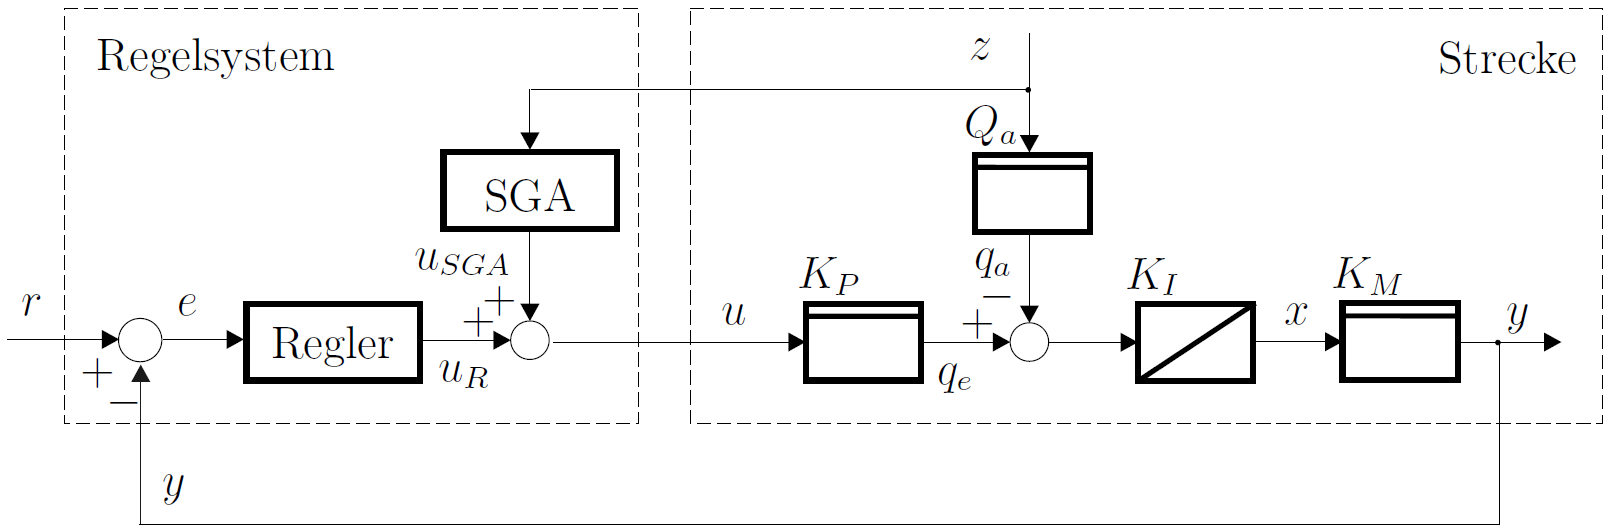
\includegraphics[width=\columnwidth]{images/stoergroessenaufschaltung.png}
    % \begin{center}
    \scalebox{0.63}{
    \begin{tikzpicture}
        [%
            scale = 1,
            >={Latex[length=1.5mm]},
            every node/.style={%
                font=\footnotesize, 
                rectangle, 
                draw, 
                minimum width=6mm, 
                minimum height=4mm
            },
            clearnode/.style={%
                rectangle, 
                draw=none, 
                fill=none, 
                minimum width=5mm, 
                minimum height=5mm, 
                inner sep=0pt
            },
            whitecircle/.style={%
                circle, 
                draw=black, 
                fill=white, 
                inner sep=0pt,
                minimum size=2mm
            },
        ]

        % nodes
        \node[clearnode]    (R)                         {$r(t)$};
        \node[fill=green]   (F)     [right=5mm of R]       {F};
        \node[whitecircle]  (A1)    [right=5mm of F]       {};
        \node[fill=orange]  (C1)    [right=5mm of A1]      {C1};   
        \node[whitecircle]  (A2)    [right=5mm of C1]      {};
        \node[fill=orange]  (C2)    [right=5mm of A2]      {C2};   
        \node[fill=yellow]  (G1)    [right=5mm of C2]      {G1};
        \node[fill=yellow]  (G2)    [right=5mm of G1]      {G2};
        \node[fill=yellow]  (H1)    [below=3mm of {$(A2.south west)!0.5!(G1.south east)$}] {H1};
        \node[fill=yellow]  (H2)    [below=3mm of H1]      {H2};
        \node[clearnode]    (U)     [right=5mm of G2]      {$u(t)$};

        % arrows
        \begin{scope}[every path/.style={->, thick}]
            \coordinate (G1G2) at ($(G1.east)!0.4!(G2.west)$);
            \coordinate (G2U) at ($(G2.east)!0.4!(U.west)$);
            
            \draw   (R)         to (F.west);
            \draw   (F.east)    to (A1.west);
            \draw   (A1.east)   to (C1.west);
            \draw   (C1.east)   to (A2.west);
            \draw   (A2.east)   to (C2.west);
            \draw   (C2.east)   to (G1.west);
            \draw   (G1.east)   to (G2.west);
            \draw   (G2.east)   to (U);
            \draw   (G1G2)      to (G1G2|-H1.east) to (H1.east); 
            \draw   (G2U)       to (G2U|-H2.east) to (H2.east); 
            \draw   (H2.west)   to (H2.west-|A1.south) to (A1.south);
            \draw   (H1.west)   to (H1.west-|A2.south) to (A2.south);
        \end{scope}
    \end{tikzpicture}}
\end{center} #TODO fix drawing
\end{minipage}
\hfill
\begin{minipage}[c]{0.43\columnwidth}
    Durch Messungen wird versucht, den Einfluss von Störungen $z(t)$ auf die Strecke gleich im Vornherein mittels 
    \cbl{SGA} zu kompensieren.
\end{minipage}

\vspace{0.2cm}

\begin{minipage}[t]{0.48\columnwidth}
    Am \cgn{grünen Knoten} gilt:
    $$ \dot{y} = K_M K_I [K_P u(t) - Q_a z(t)] $$
    Die Störung soll mittels \textbf{additiver Korrektur} des Reglerausgangs $u_R(t)$ erfolgen. 

    Aus dem Blockschaltbild ersichtlich:
    $$u(t) = u_R(t) + u_{\rm SGA}(t) $$

    $u_{\rm SGA}(t)$ soll den Einfluss von $z(t)$ am \cbl{blauen Knoten} kompensieren.
\end{minipage}
\hfill
\begin{minipage}[t]{0.48\columnwidth}
    Am \cbl{blauen Knoten} gilt:
    $$ \dot{y} = K_M K_I [K_P u_R(t) + \underbrace{ K_p u_{\rm SGA}(t) - Q_a z(t)}_{\text{soll sich auslöschen}}] $$
    Wähle $u_{\rm SGA}(t)$ so, dass die gewünschte Auslöschung stattfindet:
    $$ u_{\rm SGA}(t) = \frac{Q_a}{K_P} z(t) $$
    Somit wird die Störung kompensiert und es bleibt:
    $$ \dot{y} = K_M K_I K_P u_R(t)$$
\end{minipage}


\subsection{Kaskadenregelung}{175}

Regelstrecken 1. und 2. Ordnung ($\text{PT}_1$, $\text{PT}_2$, $I$, $\text{IT}_1$) können gut mit PID-Reglern gereglet werden. 
Bei Strecken höherer Ordnung liefert dieses Vorgehen keine genügenden Resultate mehr.

\begin{itemize}
    \item Geschlossener Regelkreis ist zu langen oder zu wenig gedämpft
    \item Einstellregeln funktionieren gar nicht, weil die Regelstrecke im offenen Betrieb immer instabil ist
\end{itemize}

\textbf{Konsequenz:} Für Strecken höherer Ordnung bracuht es auch einen Regler höherer Ordnung \textrightarrow Kaskadenregelung


\subsection{Übertragungsfunktionen Kaskadenregelung}

\begin{minipage}[c]{0.48\columnwidth}
    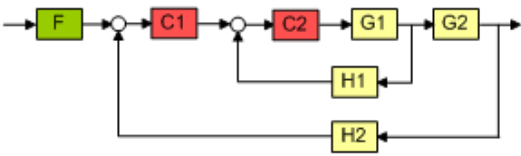
\includegraphics[width=\columnwidth]{images/kaskadenregelung_struktur.png}
    $$ \text{Annahme - Ideale Sensoren: } H_1 = H_2 = 1$$
    % \begin{center}
    \scalebox{0.63}{
    \begin{tikzpicture}
        [%
            scale = 1,
            >={Latex[length=1.5mm]},
            every node/.style={%
                font=\footnotesize, 
                rectangle, 
                draw, 
                minimum width=6mm, 
                minimum height=4mm
            },
            clearnode/.style={%
                rectangle, 
                draw=none, 
                fill=none, 
                minimum width=5mm, 
                minimum height=5mm, 
                inner sep=0pt
            },
            whitecircle/.style={%
                circle, 
                draw=black, 
                fill=white, 
                inner sep=0pt,
                minimum size=2mm
            },
        ]

        % nodes
        \node[clearnode]    (R)                         {$r(t)$};
        \node[fill=green]   (F)     [right=5mm of R]       {F};
        \node[whitecircle]  (A1)    [right=5mm of F]       {};
        \node[fill=orange]  (C1)    [right=5mm of A1]      {C1};   
        \node[whitecircle]  (A2)    [right=5mm of C1]      {};
        \node[fill=orange]  (C2)    [right=5mm of A2]      {C2};   
        \node[fill=yellow]  (G1)    [right=5mm of C2]      {G1};
        \node[fill=yellow]  (G2)    [right=5mm of G1]      {G2};
        \node[fill=yellow]  (H1)    [below=3mm of {$(A2.south west)!0.5!(G1.south east)$}] {H1};
        \node[fill=yellow]  (H2)    [below=3mm of H1]      {H2};
        \node[clearnode]    (U)     [right=5mm of G2]      {$u(t)$};

        % arrows
        \begin{scope}[every path/.style={->, thick}]
            \coordinate (G1G2) at ($(G1.east)!0.4!(G2.west)$);
            \coordinate (G2U) at ($(G2.east)!0.4!(U.west)$);
            
            \draw   (R)         to (F.west);
            \draw   (F.east)    to (A1.west);
            \draw   (A1.east)   to (C1.west);
            \draw   (C1.east)   to (A2.west);
            \draw   (A2.east)   to (C2.west);
            \draw   (C2.east)   to (G1.west);
            \draw   (G1.east)   to (G2.west);
            \draw   (G2.east)   to (U);
            \draw   (G1G2)      to (G1G2|-H1.east) to (H1.east); 
            \draw   (G2U)       to (G2U|-H2.east) to (H2.east); 
            \draw   (H2.west)   to (H2.west-|A1.south) to (A1.south);
            \draw   (H1.west)   to (H1.west-|A2.south) to (A2.south);
        \end{scope}
    \end{tikzpicture}}
\end{center}
\end{minipage}
\hfill
\begin{minipage}[c]{0.48\columnwidth}
    Übertragungsfunktion innerer Regelkreis
    $$ G_{f1} = \frac{G_1 G_2}{1 + G_1 G_2} $$
    Übertragungsfunktion äusserer Regelkreis
    $$ \textstyle{ G_{f2} = \frac{G_2 G_{f1} C_1}{1 + G_2 G_{f1} C_1} = \frac{G_2 G_1 C_2 C_1}{1 + G_1 C_2 + G_2 G_1 C_2 C_2}} $$
\end{minipage}

\vspace{0.2cm}
\textbf{Der innere Regelkreis ist deutlich schneller als der äussere Regelkreis!}

$$ G_{f1} \approx K_1 \Rightarrow G_{f2} \approx \frac{G_2 K_1 C_1}{1 + G_2 K_1 C_1} = \frac{G_3 C_1}{1 + G_3 C_1} \Rightarrow G_3 = G_2 K_1 $$

$$ G_{f1} \approx 1  \Rightarrow G_{f2} \approx \frac{G_2 C_1}{1 + G_2 C_1}  $$

\textbf{Interpretation:} Der äussere Regelkreis sieht den inneren Regelkreis nur als Verstärkung $K_1$. Wird $K_1 = 1$ gesetzt, so
ist der innere Regelkreis aus sicht des äusseren Regelkreises gar nicht vorhanden.


\subsubsection{Eigenschaften der Kaskadenregelung}

\begin{outline}
    \1 Der innere Regelkreis muss \textbf{deutlich schneller} sein, als der äussere Regelkreis
        \2 Innere Regelkreis erscheint somit für äusseren Regelkreis nur als eine \textbf{Konstante}
    \1 Der innere Regelkreis wird \textbf{zuerst} ausgelegt
        \2 Dynamik der inneren Regelstrecke verbessern (schneller machen)
        \2 Allenfalls ist eine gute Störunterdrückung wichtig ($G_z$ optimieren) % CHECK was ist mit ($G_z$ optimieren) gemeint?
    \1 Beide Regelkreise können mit \textbf{Einstellregeln} eingestellt werden
        \2 Innerer Regelkreis: Äusseren Regelkreis als offen ('nicht da') betrachten
        \2 Äusserer Regelkreis: Innerer Regelkreis muss geschlossen sein (und funktionieren)
    \1 Verfahren ist erweiterbar auf mehrstufige Kaskaden
\end{outline}


\example{Drehzahlregelung Elektromotor mit Kaskadenregelung}

\begin{minipage}[c]{0.5\columnwidth}
    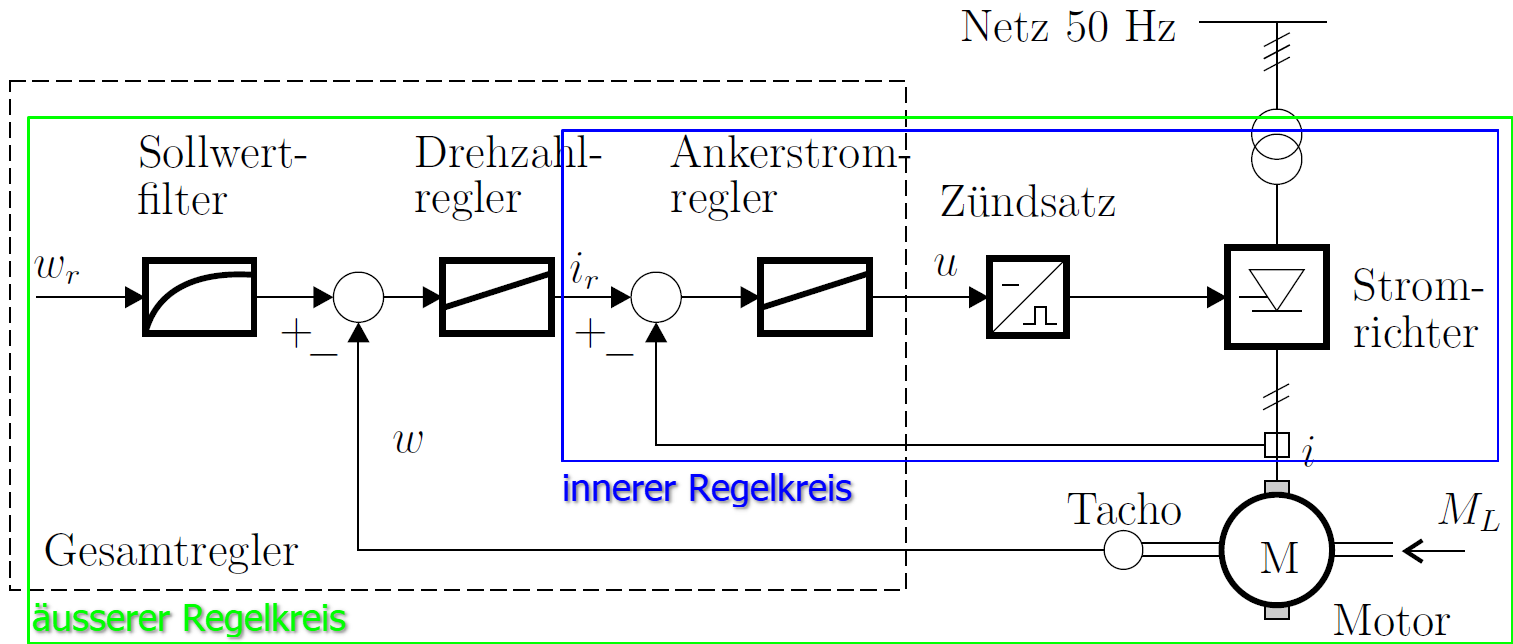
\includegraphics[width=\columnwidth]{images/kaskadenregelung_beispiel.png}
\end{minipage}
\hfill
\begin{minipage}[c]{0.48\columnwidth}
    \begin{outline}
        \1 Der innere Regelkreis regelt den Strom
            \2 Regelgrösse $r_1(t)$: Strom
            \2 Stellgrösse $u_1(t)$: Spannung
        \1 Der äussere Regler regelt die Drehzahl
        \2 Regelgrösse $r(t)$: Drehzahl
        \2 Stellgrösse $u(t) = r_1(t)$: Strom
    \end{outline}
\end{minipage}


% \subsection{Wind-Up}